\section{Experiments and Results}
We use transactional data from instacart kaggle challenge to train all our models. A preview of data used is 
shown in Figure~\ref{fig:sampledata}. 

For simplicity and better generalization we adopted non-parameteric approach for stacking.
We used Weighted K Best Stacked Generalization Ensemble for combining the 60 models (candidates) from Table 1. 
Test1 Logloss was used as metric to compute weight for each of the 46 candidates. We set the k to 25 and selected 
these top 25 candidates based upon the experiments performed over test1 metrics. Finally, we took Weighted Average of 
the probabilities for Validation, Test1 and Test2 time steps for each consumer-item combination.
For simplicity and better generalization we adopted non-parameteric approach for stacking.
We used Weighted K Best Stacked Generalization Ensemble for combining the 60 models (candidates) from Table 1. 
Test1 Logloss was used as metric to compute weight for each of the 46 candidates. We set the k to 25 and selected 
these top 25 candidates based upon the experiments performed over test1 metrics. Finally, we took Weighted Average of 
the probabilities for Validation, Test1 and Test2 time steps for each consumer-item combination.

 \begin{figure}[t]
    \centering 
    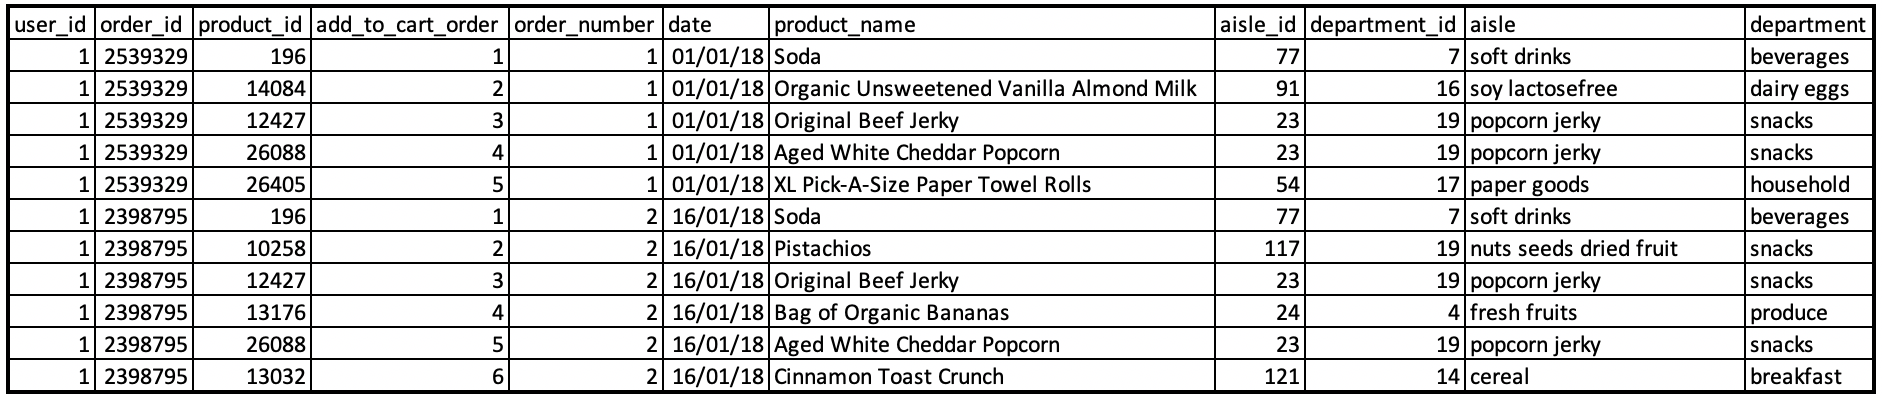
\includegraphics[width=3.3in]{img/sampledata.png} 
    \caption{Sample Dataset} 
    \label{fig:sampledata} 
  \end{figure}

  \begin{figure}[t]
    \centering 
    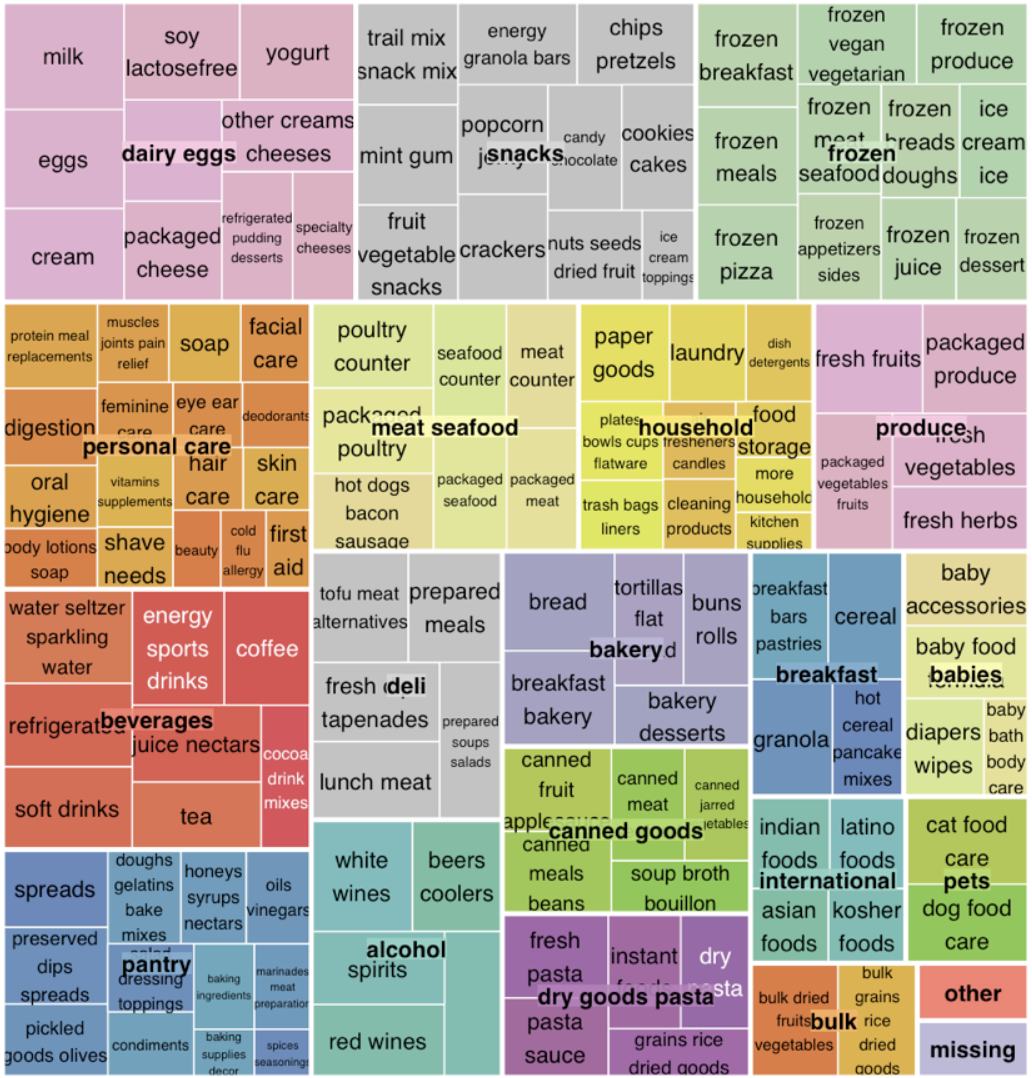
\includegraphics[width=3.3in]{img/items.png} 
    \caption{Most ordered items} 
    \label{fig:items} 
  \end{figure}

  \begin{figure}[t]
    \centering 
    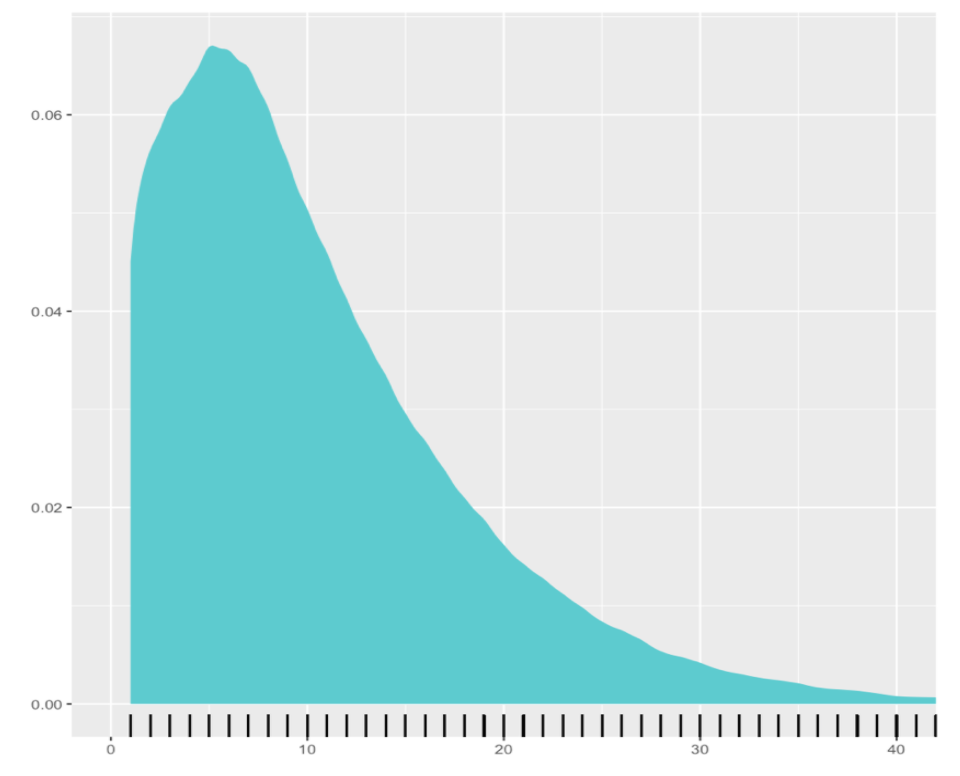
\includegraphics[width=3.3in]{img/basket.png} 
    \caption{Density of consumers Vs. Basket Size} 
    \label{fig:basket} 
  \end{figure}

  \begin{figure}[t]
    \centering 
    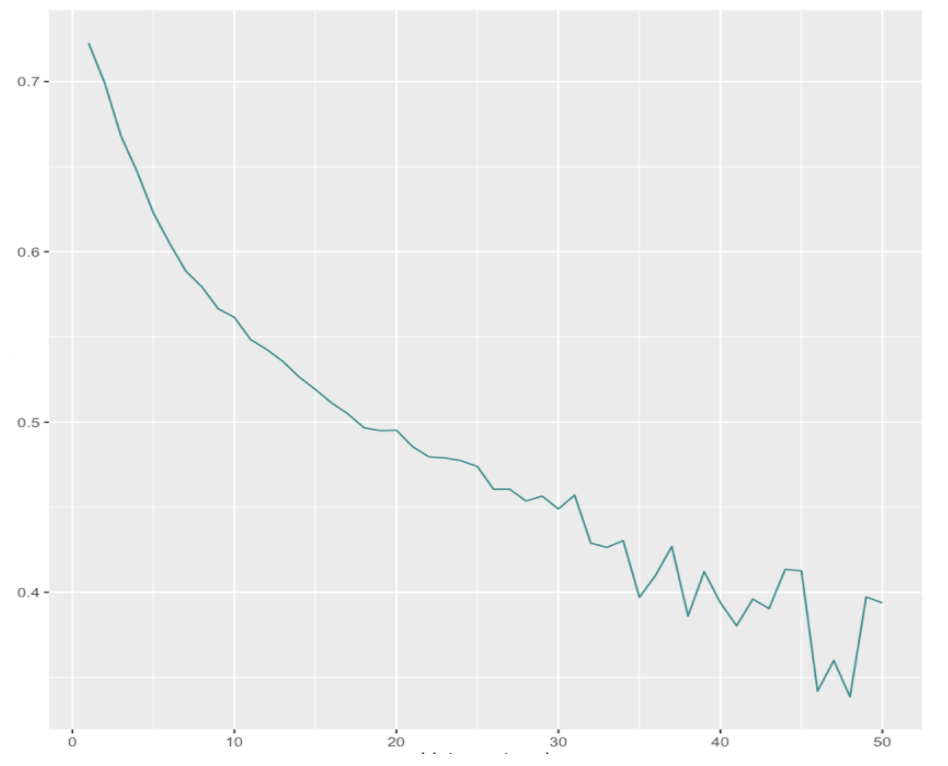
\includegraphics[width=3.3in]{img/addtocart.png} 
    \caption{Order probability Vs. Add to cart order} 
    \label{fig:basket} 
  \end{figure}


\begin{table}[t]
\caption{ Training Results}
\vspace{0.1 in}
\centering
\resizebox{3.3in}{!}
{%
\begin{tabular}{|c|c|c|c|}
\hline
{\bf Model Type} & {\bf Val BCELoss} & {\bf Test1 BCELoss} & {\bf Test2 BCELoss} \\  \hline
MLP	  		&  0.18 &  0.18 &  0.18  \\ \hline
LSTM  		&  0.17 &  0.17 &  0.17 \\ \hline
TCN			&  0.15  &  0.15 &  0.15  \\ \hline
TCNLSTM 	& 0.13  & 0.13	& 0.13	 \\ \hline
Xgboost 	& 0.21 & 0.21	& 0.21	\\ \hline
RandomForest & 0.23 & 0.23	& 0.23	\\ \hline
\end{tabular}
}
\label{tab:training}
\end{table}


\begin{table}[t]
\caption{ Stacked Generalization Results}
\vspace{0.1 in}
\centering
\resizebox{3.3in}{!}
{%
\begin{tabular}{|c|c|c|c|c|}
\hline
{\bf Model Type} & {\bf K Value} & {\bf Val BCELoss} & {\bf Test1 BCELoss} & {\bf Test2 BCELoss} \\  \hline
Weighted K Best	  		&  5 &  0.18 &  0.18 &  0.18  \\ \hline
Weighted K Best	  		&  10 &  0.18 &  0.18 &  0.18  \\ \hline
Weighted K Best	  		&  25 &  0.18 &  0.18 &  0.18  \\ \hline
K Best	  		&  3 &  0.18 &  0.18 &  0.18  \\ \hline
K Best	  		&  5 &  0.18 &  0.18 &  0.18  \\ \hline
\end{tabular}
}
\label{tab:stacking}
\end{table}